\documentclass{article}\usepackage{graphicx}\date{\today}\setlength{\textwidth}{7.1in}\setlength{\oddsidemargin}{-0.4in}\setlength{\textheight}{9.6in}\setlength{\topmargin}{-0.8in}\begin{document}\today\section*{ Convergence report for Bone Benign signatures ROO RData} Date of inference: 2020-06-13\\\textbf{Explanation of parameters} Rhat indicates the ratio of variance within a change over variance pooling all chains. \emph{We recommend running at least four chains by default and only using the sample if R-hat is less than 1.05.} ESS bulk/tail indicate the bulk/tail effective sample size estimate, i.e. show the sampling efficiency of mean and median estimates. \emph{We recommend running at least four chains by default and only using the sample if R-hat is less than 1.05. Both bulk-ESS and tail-ESS should be at least 100 (approximately) per Markov Chain in order to be reliable and indicate that estimates of respective posterior quantiles are reliable.}\begin{itemize}\item Max Rhat: 1.00039451676644
\item ess bulk: 130.367381603145
\item ess tail: 147.746002326617\end{itemize}
\begin{minipage}{\textwidth}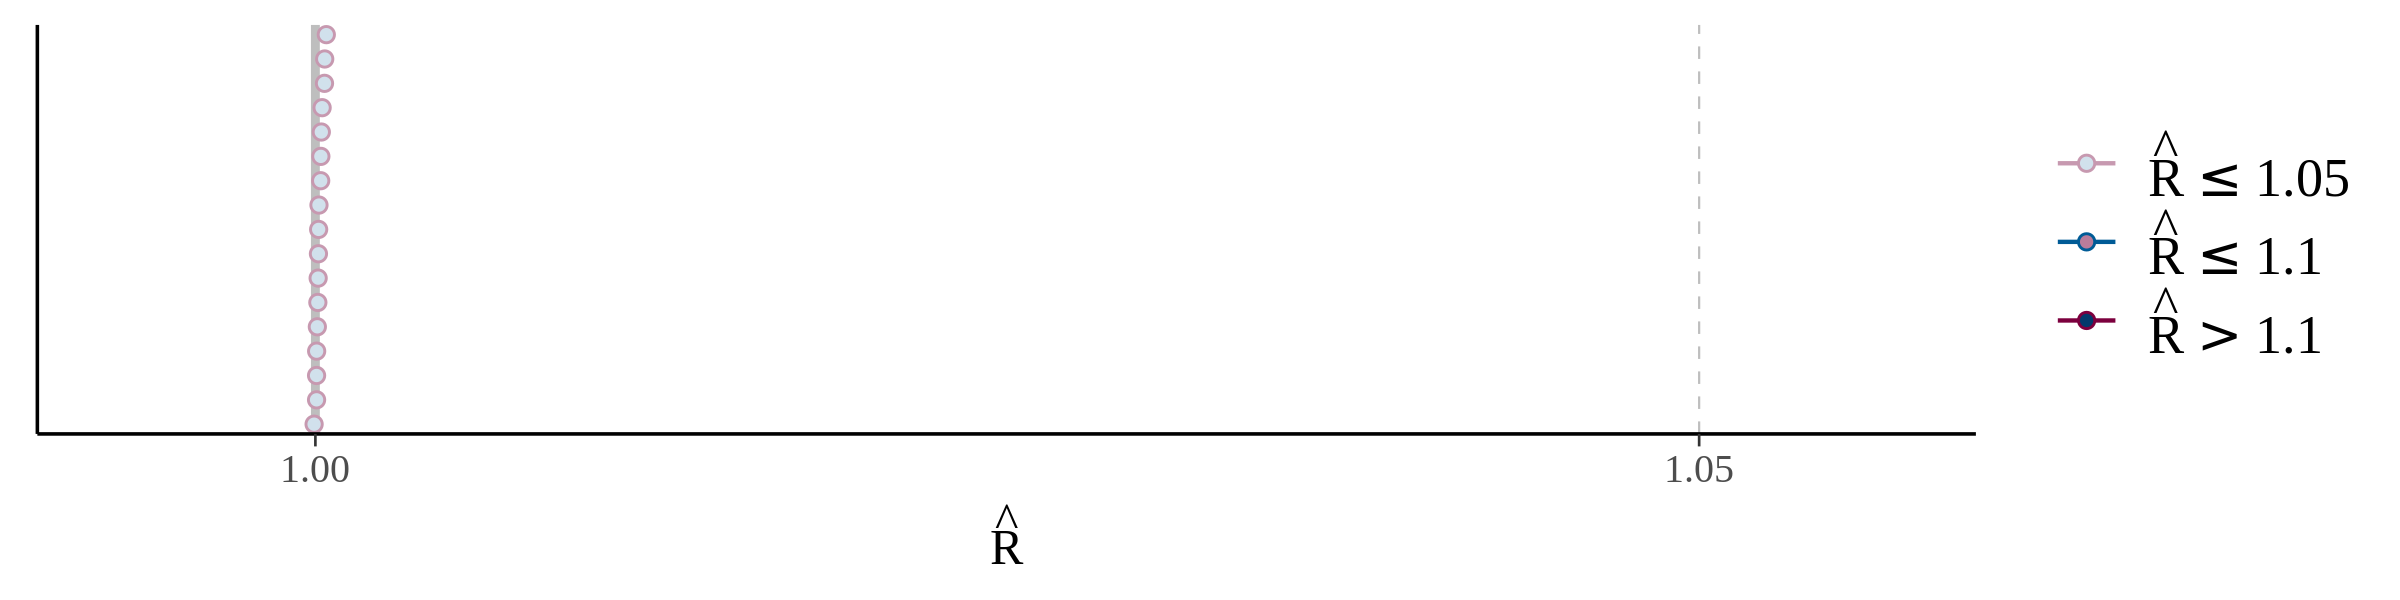
\includegraphics[width=\textwidth]{../figures/Bone_Benign_signatures_ROO_RDatamcmc_rhat.png}\end{minipage}\\In the plots below ESS should have high values\\\begin{minipage}{.3\textwidth}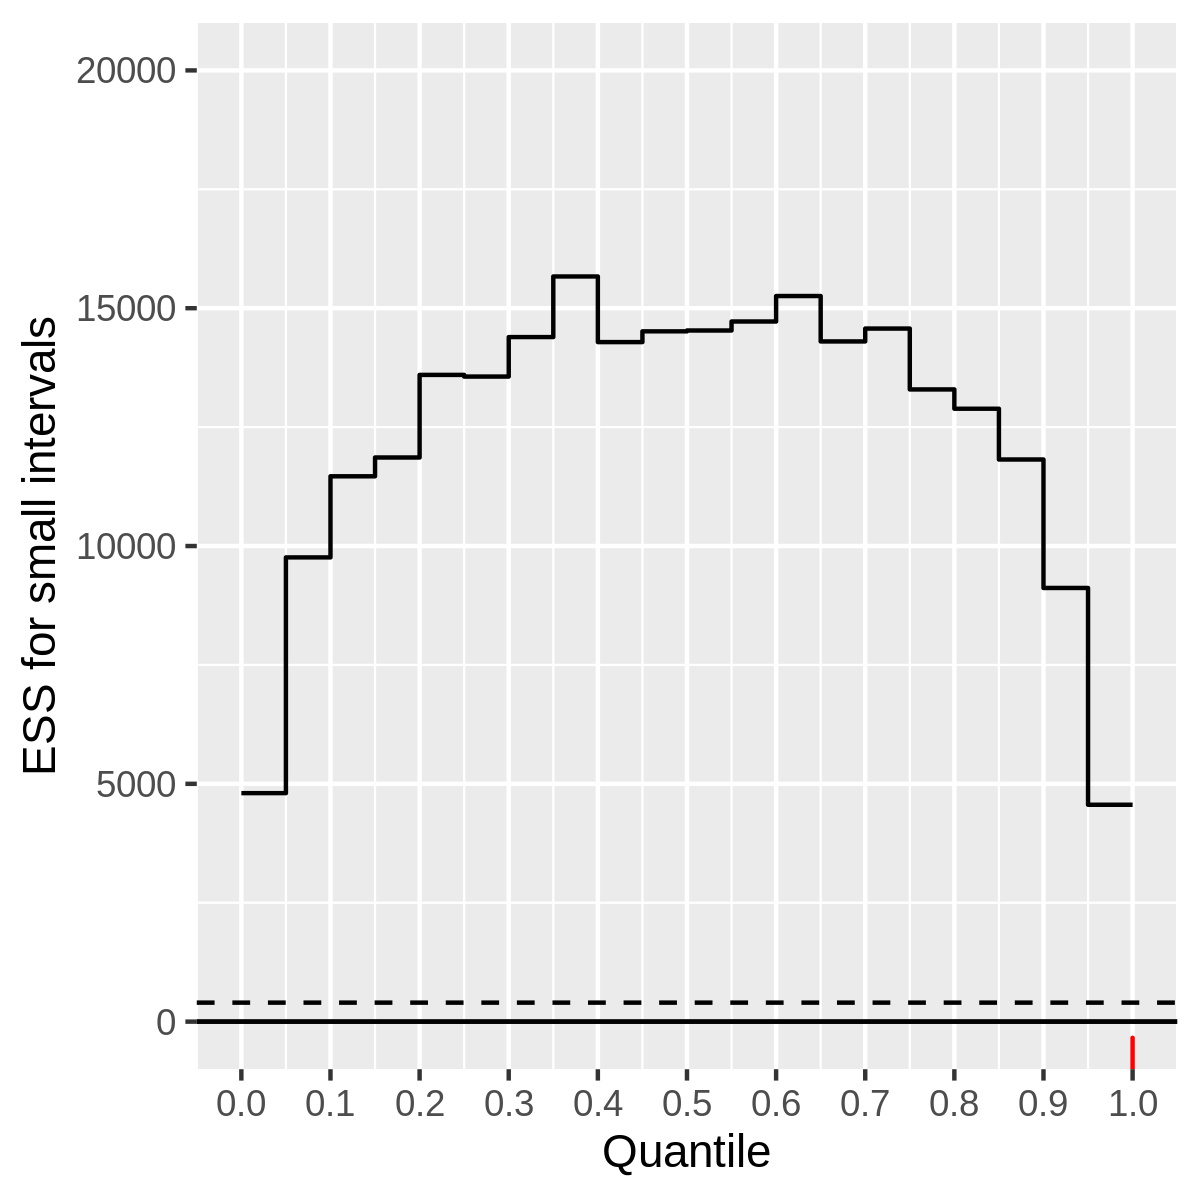
\includegraphics[width=\textwidth]{../figures/Bone_Benign_signatures_ROO_RDatalocal_ess_min.png}\end{minipage}\begin{minipage}{.3\textwidth}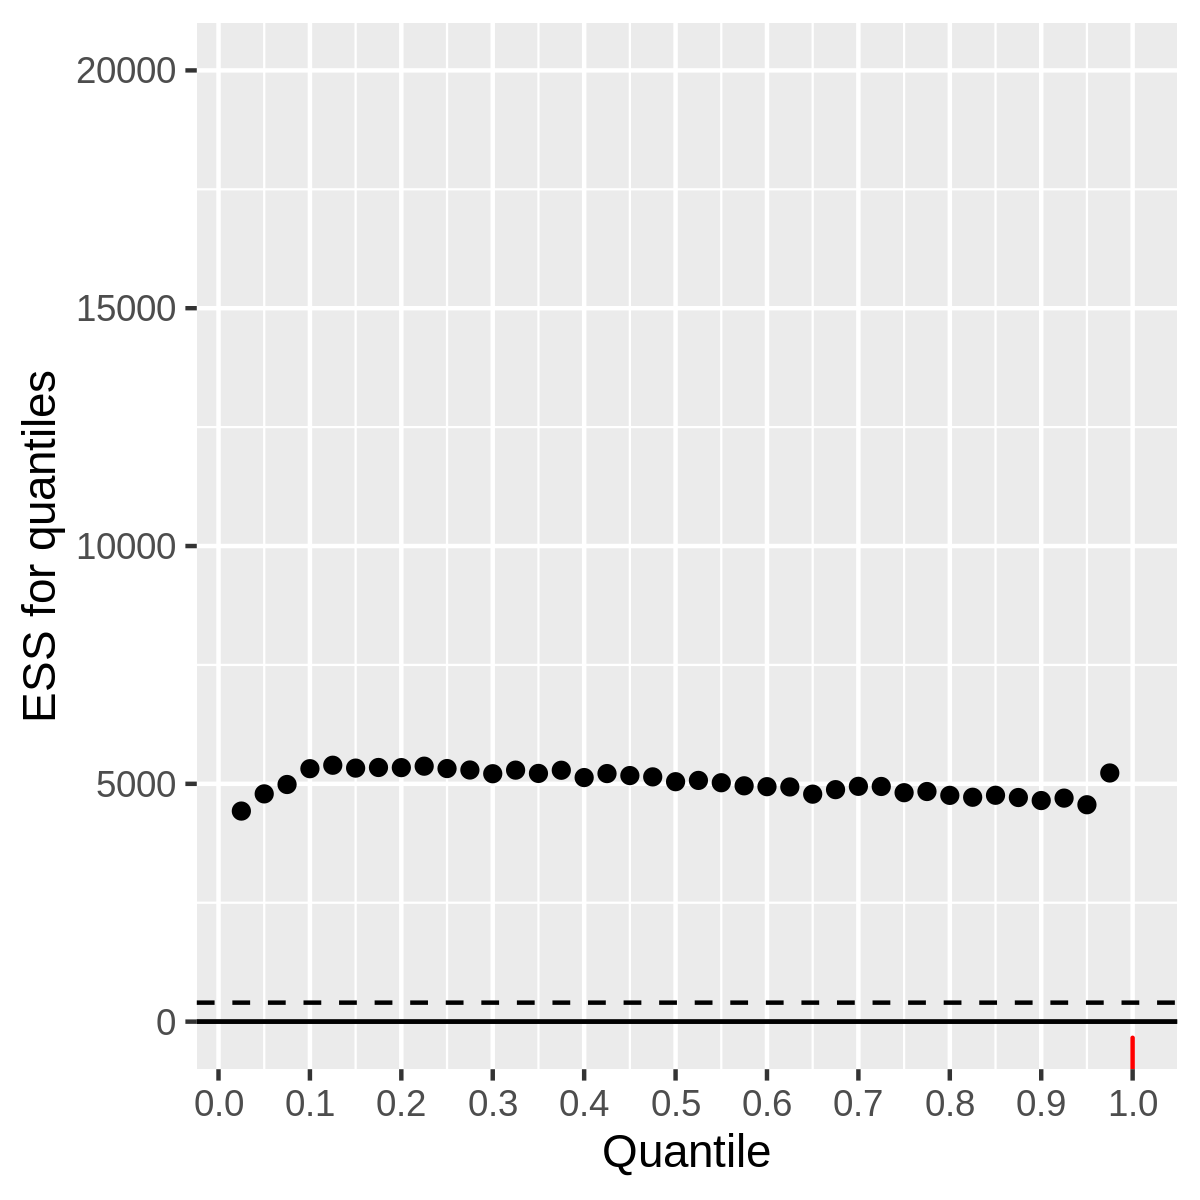
\includegraphics[width=\textwidth]{../figures/Bone_Benign_signatures_ROO_RDataquantile_ess.png}\end{minipage}\begin{minipage}{.36\textwidth}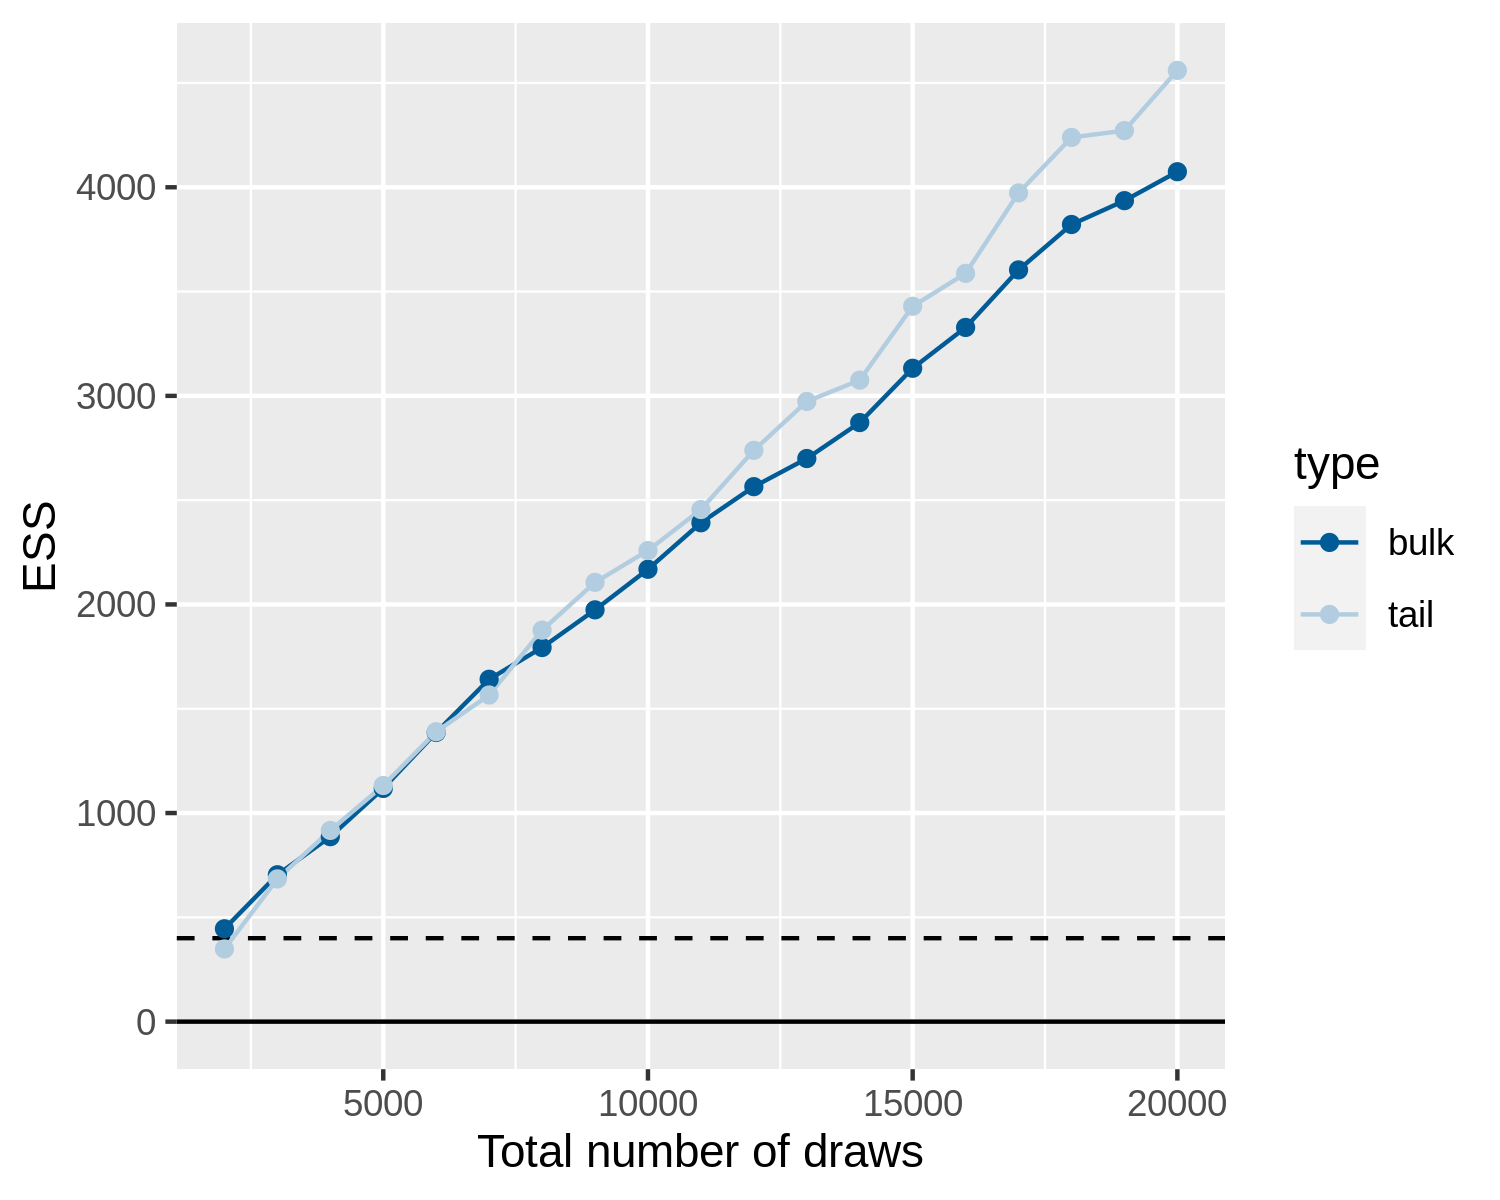
\includegraphics[width=\textwidth]{../figures/Bone_Benign_signatures_ROO_RDataquantile_ess_min.png}\end{minipage}
\subsection*{Local ESS for $\beta$}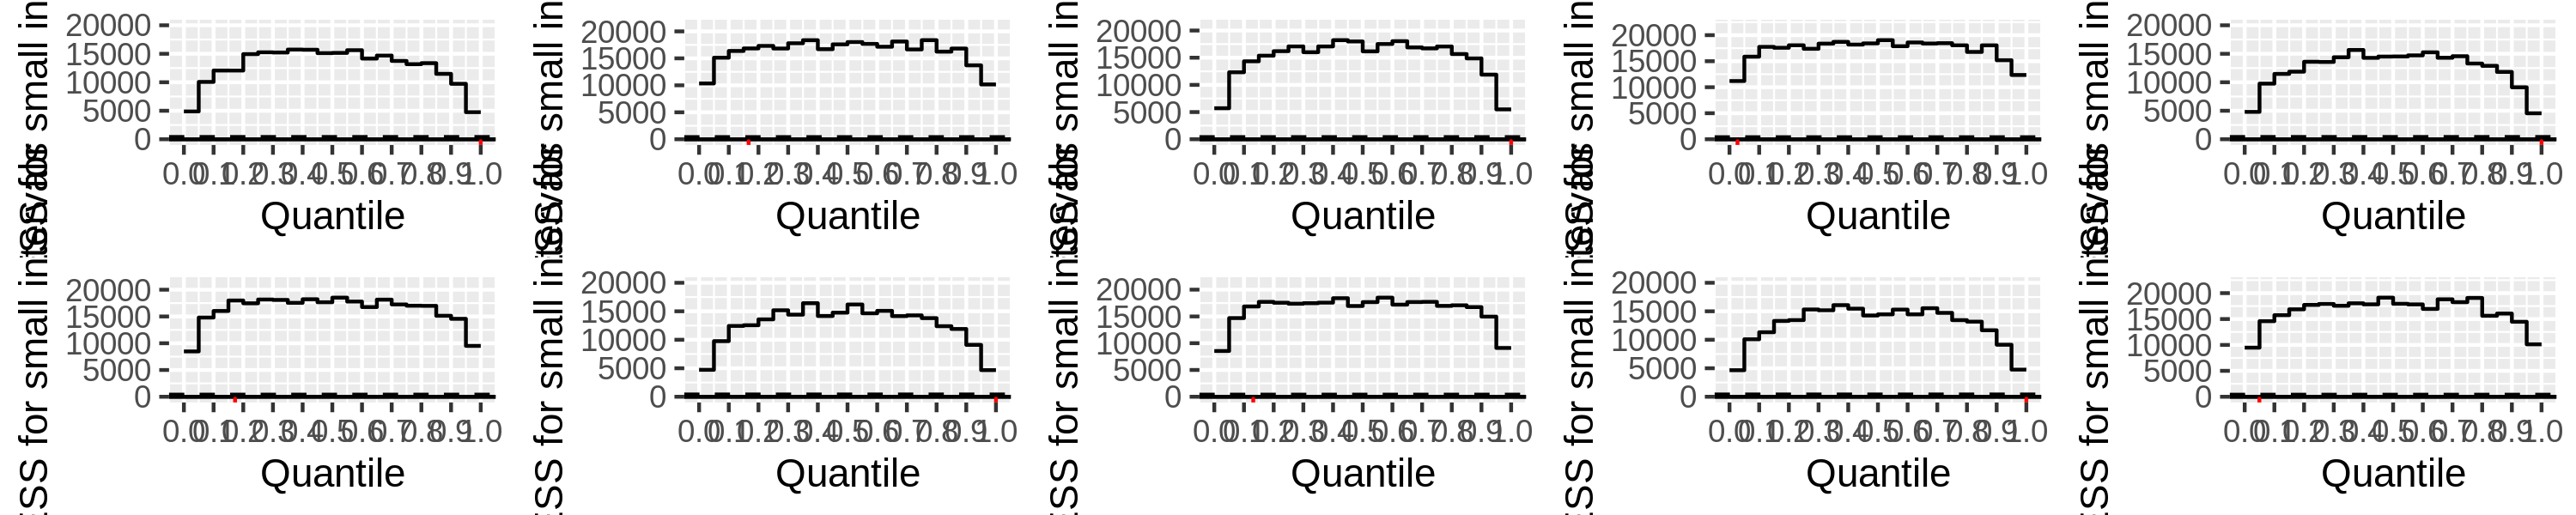
\includegraphics[width=\textwidth]{../figures/Bone_Benign_signatures_ROO_RDatalocal_ess_beta.png}
\end{document}
